\documentclass[11pt,a4paper]{article}

% Packages - load hyperref LAST for proper citation linking
\usepackage[utf8]{inputenc}
\usepackage[T1]{fontenc}
\usepackage{geometry}
\geometry{margin=1in}
\usepackage{setspace}
\onehalfspacing
\usepackage{graphicx}
\usepackage{booktabs}
\usepackage{amsmath}
\usepackage{caption}
\usepackage{subcaption}
\usepackage{array}
\usepackage{longtable}
\usepackage{url}
\usepackage[numbers,sort&compress]{natbib}
\usepackage[colorlinks=true,linkcolor=blue,citecolor=blue,urlcolor=blue]{hyperref}
\usepackage{multirow}
\usepackage{float}

% Title and author information
\title{\textbf{Comorbidity Burden, Micronutrient Intake, and Balance Performance in Older Adults:} \\ \textbf{NHANES 2003-2004}}

\author{Elwood Research\\
\texttt{elwoodresearch@gmail.com}}

\date{February 2026}

\begin{document}

\maketitle

% Abstract
\begin{abstract}
\noindent\textbf{Background:} Falls and balance impairment represent significant public health concerns among older adults, with comorbidity burden and nutritional status identified as potential risk factors. Despite theoretical links between polypharmacy, micronutrient status, and physical function, few studies have examined how comorbidity burden and dietary micronutrients jointly influence objective balance performance in community-dwelling older adults.

\noindent\textbf{Methods:} We conducted a cross-sectional analysis of 788 adults aged 60+ years from NHANES cycle C (2003-2004). Comorbidity burden was operationalized as a count of cardiometabolic conditions (diabetes, hypertension, hypercholesterolemia). Dietary micronutrient intake (vitamin B12, folate) was derived from 24-hour dietary recalls. The primary outcome was balance failure time on the modified Romberg test (BAXFTC41). Survey-weighted linear regression models tested main effects and interactions, adjusting for age, sex, BMI, and dietary energy intake.

\noindent\textbf{Results:} The final analytic sample of 788 participants (weighted mean age 70.9 years, 42.7\% male) had a mean comorbidity burden of 1.33 conditions. Neither comorbidity burden ($\beta$=-0.032, p=0.340) nor dietary micronutrients (vitamin B12: $\beta$=0.039, p=0.215; folate: $\beta$=0.015, p=0.627) demonstrated significant associations with balance performance. Interaction terms between comorbidity burden and micronutrients were also non-significant. Age emerged as the only significant predictor ($\beta$=-0.020, p$<$0.001), with older age associated with shorter balance failure times.

\noindent\textbf{Conclusions:} In this nationally representative sample of older adults, comorbidity burden and dietary micronutrient intake (B12, folate) were not significantly associated with objective balance performance. The predominance of age as a predictor suggests that chronological aging processes may overshadow the effects of comorbidity and dietary intake within the observed ranges. These null findings highlight methodological challenges in assessing micronutrient-balance relationships using dietary intake data and underscore the need for biomarker-based assessment in future research.

\vspace{0.3cm}
\noindent\textbf{Keywords:} comorbidity, polypharmacy, vitamin B12, folate, balance, falls, older adults, NHANES, physical function
\end{abstract}

% Introduction
\section{Introduction}

Balance impairment and falls represent critical public health concerns among older adults, contributing substantially to morbidity, mortality, and healthcare costs. Approximately one-third of community-dwelling adults aged 65 and older experience at least one fall annually, with fall-related injuries leading to over 3 million emergency department visits and 800,000 hospitalizations each year in the United States \cite{talkowski2008_balance_gait_walking}. Given the aging demographic profile of developed nations, understanding modifiable risk factors for balance impairment has become increasingly urgent.

\subsection{Comorbidity Burden and Balance}

The relationship between chronic disease burden and physical function has been well-documented. Multiple chronic conditions, often accompanied by polypharmacy, have been associated with reduced physical performance, increased disability, and elevated fall risk \cite{katsimpris2019_polypharmacy_function_review}. A systematic review by Katsimpris et al. \cite{katsimpris2019_polypharmacy_function_review} identified consistent associations between polypharmacy and lower physical function across multiple measures, including gait speed, chair stand tests, and self-reported disability. Salkin et al. \cite{salkin2025_polypharmacy_balance} reported that older adults with polypharmacy demonstrated significantly poorer Berg Balance Scale scores and slower Timed Up and Go performance compared to those on fewer medications.

The mechanisms linking comorbidity burden to balance impairment are multifactorial. Cardiometabolic conditions such as diabetes and hypertension can affect balance through peripheral neuropathy, orthostatic hypotension, and reduced proprioceptive function \cite{romandemettelinge2013_diabetes_falls_medications}. Additionally, the medications used to treat chronic conditions—particularly central nervous system-active drugs—may directly impair balance and cognition, creating iatrogenic risk that compounds disease-related impairment.

\subsection{Micronutrients and Physical Function}

Micronutrient status represents another potential determinant of balance and physical function in older adults. Vitamin B12 and folate play essential roles in neurological function, myelin maintenance, and homocysteine metabolism, with deficiency states associated with peripheral neuropathy, cognitive impairment, and gait abnormalities \cite{vidoni2017_b12_hcy_gait, ng2012_b12_folate_function}.

Observational studies have documented associations between B12-related metabolic pathways and physical performance. Kositsawat et al. \cite{kositsawat2022_nhanes_hcy_function} reported that elevated plasma homocysteine—a marker of B12/folate metabolism—was independently associated with slower gait speed and lower grip strength in NHANES participants. Ji et al. \cite{ji2023_nhanes_folate_disability} found that higher serum folate concentrations were associated with lower odds of functional disability across multiple domains. Vidoni et al. \cite{vidoni2017_b12_hcy_gait} demonstrated associations between vitamin B12, homocysteine, and gait speed in the Baltimore Longitudinal Study of Aging.

Vitamin D has also been extensively studied in relation to balance and physical performance. Multiple NHANES-based studies have documented associations between serum 25-hydroxyvitamin D and gait speed, functional disability, and physical performance \cite{orces2019_nhanes_vitd_disability, kalenkoski2020_nhanes_vitd_gait}, while cohort studies such as InCHIANTI have demonstrated relationships between vitamin D and lower-extremity performance \cite{shardell2015_vitd_klotho_performance}. Moon et al. \cite{moon2019_vitd_performance} specifically reported associations between 25(OH)D levels and physical performance tests in community-dwelling older adults.

\subsection{Potential Interactions}

The potential for micronutrient status to modify the relationship between comorbidity burden and balance has received limited attention. Emerging evidence suggests that nutritional factors may interact with disease burden and inflammatory status to influence physical function. Kositsawat et al. \cite{kositsawat2019_vitd_il6_gait} demonstrated a vitamin D × interleukin-6 interaction on gait speed in the InCHIANTI cohort, suggesting that micronutrient effects may be most pronounced among individuals with elevated inflammatory burden—a common consequence of chronic disease.

This potential effect modification has important clinical implications. If low micronutrient status exacerbates balance impairment among older adults with high comorbidity burden, targeted nutritional interventions could represent a modifiable pathway for fall prevention in this vulnerable population. Conversely, adequate micronutrient status may buffer against the detrimental effects of chronic disease on physical function.

\subsection{Study Objectives}

Given the established independent relationships between comorbidity burden, micronutrient status, and physical function, we examined whether these factors jointly influence objective balance performance in a nationally representative sample of US older adults. Our primary objectives were to: (1) quantify associations between comorbidity burden and balance performance; (2) evaluate main effects of dietary micronutrient intake (vitamin B12, folate) on balance; and (3) test whether micronutrient status modifies the relationship between comorbidity burden and balance outcomes.

% Methods
\section{Methods}

\subsection{Study Design and Data Source}

We conducted a cross-sectional analysis of NHANES cycle C (2003-2004). NHANES employs a complex, multistage, probability sampling design to produce nationally representative estimates of the non-institutionalized US population. The survey protocol was approved by the National Center for Health Statistics Ethics Review Board, and all participants provided informed consent.

\subsection{Study Population}

Inclusion criteria were: age $\geq$60 years at screening; completion of the balance examination with valid failure time data for the most challenging condition; valid dietary recall data (day 1); and complete survey design variables. We excluded participants missing balance subsample weights (WTSB2YR) or survey design variables (SDMVPSU, SDMVSTRA).

\subsection{Outcomes: Balance Performance}

Balance outcomes were derived from the BAX\_C examination dataset. The primary outcome was failure time in seconds for the most challenging balance condition (BAXFTC41), representing the ability to maintain a tandem stance with eyes closed on a foam surface. This modified Romberg test assesses the integration of vestibular, visual, and proprioceptive systems critical for postural control. Secondary outcomes included pass/fail indicators for each balance condition (BAXPFC11, BAXPFC21, BAXPFC31, BAXPFC41).

\subsection{Exposures}

\subsubsection{Comorbidity Burden}

Comorbidity burden was constructed as a count (0-3) of self-reported cardiometabolic conditions from the diabetes (DIQ\_C) and blood pressure/cholesterol (BPQ\_C) questionnaires:
\begin{itemize}
    \item Diabetes (DIQ010): Participant reported being told by a doctor they had diabetes
    \item Hypertension (BPQ020): Participant reported being told they had high blood pressure
    \item High cholesterol (BPQ080): Participant reported being told they had high cholesterol
\end{itemize}
The count was analyzed as a continuous exposure (0-3) and categorized as 0, 1, and 2+ conditions for interpretability.

\subsubsection{Micronutrient Intake}

Dietary micronutrient intake was obtained from DR1TOT\_C (day 1 dietary recall totals):
\begin{itemize}
    \item Vitamin B12: DR1TVB12 (mcg/day)
    \item Folate (as dietary folate equivalents): DR1TFDFE (mcg/day)
\end{itemize}
Primary analyses used continuous intake measures standardized to mean=0, SD=1. For visualization and interaction interpretation, we also evaluated tertiles of intake and energy-adjusted intake per 1,000 kcal (DR1TKCAL).

\textbf{Note:} Vitamin D intake data was unavailable in NHANES cycle C. Dietary supplement data was also unavailable for this cycle, restricting analyses to dietary micronutrient intake only.

\subsection{Covariates}

Models adjusted for demographic and health-related covariates:
\begin{itemize}
    \item Demographics: Age (RIDAGEYR, continuous), sex (RIAGENDR), race/ethnicity (RIDRETH1)
    \item Socioeconomic: Education (DMDEDUC2), income-to-poverty ratio (INDFMPIR)
    \item Health: Body mass index (BMXBMI, continuous)
    \item Dietary: Energy intake (DR1TKCAL, continuous)
\end{itemize}

\subsection{Survey Design and Weights}

All analyses incorporated NHANES survey design variables (SDMVPSU, SDMVSTRA). The balance exam uses a subsample design; we applied WTSB2YR as the primary analysis weight. Survey-weighted estimation procedures produced population-representative estimates with robust standard errors accounting for the complex sampling design.

\subsection{Data Cleaning and Exclusion Rules}

\textbf{Outlier screening:} For all continuous variables, we computed z-scores and removed observations with $|z| > 4$ prior to modeling. This rule excluded extreme values that could exert undue influence on regression estimates.

\textbf{Categorical level exclusion:} For categorical variables, levels with $<$5\% membership were excluded to avoid unstable estimates and model convergence issues.

\subsection{Statistical Analysis}

We fit survey-weighted regression models to evaluate associations between comorbidity burden, micronutrient intake, and balance outcomes:

\textbf{Continuous outcomes:} Survey-weighted linear regression for failure time. The primary model specification was:
\begin{equation}
\begin{split}
\text{Balance Time} = \beta_0 &+ \beta_1(\text{Comorbidity Count}) + \beta_2(\text{B12}) + \beta_3(\text{Folate}) \\
&+ \beta_4(\text{Age}) + \beta_5(\text{Sex}) + \beta_6(\text{BMI}) + \beta_7(\text{Energy}) + \epsilon
\end{split}
\end{equation}

\textbf{Interaction terms:} To test effect modification, we included interaction terms between comorbidity burden and each micronutrient:
\begin{equation}
\begin{split}
\text{Balance Time} = \beta_0 &+ \beta_1(\text{Comorbidity}) + \beta_2(\text{B12}) + \beta_3(\text{Comorbidity} \times \text{B12}) \\
&+ \beta_4(\text{Folate}) + \beta_5(\text{Comorbidity} \times \text{Folate}) + \text{covariates} + \epsilon
\end{split}
\end{equation}

\textbf{Binary outcomes:} Survey-weighted logistic regression for pass/fail indicators.

\subsection{Sensitivity Analyses}

We conducted sensitivity analyses to assess robustness: (1) alternative comorbidity burden parameterizations (0-3 count vs 0/1/2+ categories); (2) energy-adjusted micronutrient intake (per 1,000 kcal) vs absolute intake; and (3) excluding participants who did not meet balance readiness screening criteria (BAQ110, BAQ130).

\subsection{Reporting Standards}

We constructed a STROBE flow diagram detailing sample selection, exclusions (including outlier removal and categorical exclusions), and the final analytic sample. All methods and results were reported in accordance with STROBE recommendations for cross-sectional studies.

% Results
\section{Results}

\subsection{Sample Derivation}

Figure~\ref{fig:strobe} presents the STROBE flow diagram detailing sample selection and exclusions. The analytic sample derivation proceeded through multiple stages:

\begin{itemize}
    \item Initial merge (BAX\_C + DEMO\_C): 3,086 participants
    \item Age 60+ years: 1,750 participants
    \item Balance exam complete: 1,343 participants
    \item Valid balance outcome (BAXFTC41): 930 participants
    \item Valid survey design variables: 930 participants
    \item Valid comorbidity data: 812 participants
    \item Valid micronutrient data: 802 participants
    \item After outlier removal ($|z| > 4$): \textbf{788 participants}
\end{itemize}

The final analytic sample of 788 participants represents 25.5\% of the initial merged dataset and 45.0\% of adults aged 60+ with balance exam data. This substantial attrition reflects the strict eligibility criteria for the balance examination and the exclusion of participants with missing data on key variables.

\begin{figure}[htbp]
\centering
\fbox{\parbox{0.9\textwidth}{
\centering
\textbf{STROBE Flow Diagram}\\[0.5em]
\begin{tabular}{l|c}
\toprule
\textbf{Step} & \textbf{N} \\
\midrule
Initial merge (BAX\_C + DEMO\_C) & 3,086 \\
Age 60+ years & 1,750 \\
Balance exam complete & 1,343 \\
Valid balance outcome (BAXFTC41) & 930 \\
Valid survey design variables & 930 \\
Valid comorbidity data & 812 \\
Valid micronutrient data & 802 \\
After outlier removal ($|z| > 4$) & \textbf{788} \\
\bottomrule
\end{tabular}
}}
\caption{STROBE flow diagram showing sample derivation and exclusions. The final analytic sample includes 788 participants after sequential application of inclusion criteria and outlier removal.}
\label{fig:strobe}
\end{figure}

\subsection{Sample Characteristics}

Table~\ref{tab:characteristics} presents weighted descriptive statistics for the final analytic sample. The mean age was 70.9 years (SD 7.1), with 42.7\% male and 57.3\% female participants. The racial/ethnic distribution was predominantly Non-Hispanic White (83.6\%), with smaller proportions of Non-Hispanic Black (6.1\%) and Hispanic (5.2\%) participants.

\begin{table}[htbp]
\centering
\caption{Sample Characteristics (NHANES 2003-2004, Weighted)}
\label{tab:characteristics}
\begin{tabular}{lcc}
\toprule
\textbf{Characteristic} & \textbf{Mean/\%} & \textbf{SE/SD} \\
\midrule
\multicolumn{3}{l}{\textit{Demographics}} \\
Age (years) & 70.9 & 7.1 \\
\quad Male & 42.7\% & -- \\
\quad Female & 57.3\% & -- \\
\quad Non-Hispanic White & 83.6\% & -- \\
\quad Non-Hispanic Black & 6.1\% & -- \\
\quad Hispanic & 5.2\% & -- \\
\midrule
\multicolumn{3}{l}{\textit{Health Characteristics}} \\
BMI (kg/m$^2$) & 27.8 & 5.0 \\
Comorbidity burden & 1.33 & 0.88 \\
\quad 0 conditions & 18.5\% & -- \\
\quad 1 condition & 40.4\% & -- \\
\quad 2+ conditions & 41.1\% & -- \\
\midrule
\multicolumn{3}{l}{\textit{Micronutrient Intake (Dietary Only)}} \\
Vitamin B12 (mcg/day) & 4.50 & 3.69 \\
Folate DFE (mcg/day) & 482.21 & 256.04 \\
Energy intake (kcal/day) & 1,847 & 621 \\
\midrule
\multicolumn{3}{l}{\textit{Balance Outcome}} \\
Failure time, BAXFTC41 (seconds) & 7.01 & 5.65 \\
\bottomrule
\end{tabular}
\begin{flushleft}
\footnotesize{Note: N=788. All estimates incorporate NHANES survey weights (WTSB2YR) for population-representative inference. BMI = body mass index; DFE = dietary folate equivalents.}
\end{flushleft}
\end{table}

Health characteristics revealed a mean BMI of 27.8 kg/m$^2$ (SD 5.0), consistent with overweight status. Comorbidity burden averaged 1.33 conditions (SD 0.88), with 18.5\% reporting no conditions, 40.4\% reporting one condition, and 41.1\% reporting two or more conditions.

Dietary micronutrient intake averaged 4.50 mcg/day (SD 3.69) for vitamin B12 and 482.21 mcg/day (SD 256.04) for folate (as dietary folate equivalents). Mean energy intake was 1,847 kcal/day (SD 621).

The primary balance outcome, failure time on the most challenging condition (BAXFTC41), averaged 7.01 seconds (SD 5.65), reflecting substantial variability in balance performance within this older adult sample.

\subsection{Regression Results}

\subsubsection{Main Effects Model}

Table~\ref{tab:regression} presents survey-weighted linear regression results for the main effects model. After adjusting for age, sex, BMI, and dietary energy intake, neither comorbidity burden nor micronutrient intake demonstrated significant associations with balance performance:

\begin{itemize}
    \item \textbf{Comorbidity burden:} $\beta$ = -0.032, p = 0.340 (95\% CI: -0.097 to 0.034)
    \item \textbf{Vitamin B12:} $\beta$ = 0.039, p = 0.215 (95\% CI: -0.023 to 0.106)
    \item \textbf{Folate:} $\beta$ = 0.015, p = 0.627 (95\% CI: -0.046 to 0.076)
\end{itemize}

\textbf{Age} emerged as the only statistically significant predictor ($\beta$ = -0.020, p $<$ 0.001, 95\% CI: -0.028 to -0.013), with each additional year of age associated with approximately 0.02 seconds shorter balance failure time—indicating worse balance performance with advancing age. Over a 10-year age difference, this translates to approximately 0.2 seconds shorter failure time, or roughly 3\% reduction from the mean.

Sex showed a marginally significant association ($\beta$ = -0.099, p = 0.084), with female sex associated with slightly worse balance performance. BMI was not significantly associated with balance outcomes ($\beta$ = 0.010, p = 0.113).

\begin{table}[htbp]
\centering
\caption{Survey-Weighted Linear Regression Results: Predictors of Balance Performance}
\label{tab:regression}
\begin{tabular}{lcccc}
\toprule
\textbf{Variable} & \textbf{$\beta$} & \textbf{SE} & \textbf{95\% CI} & \textbf{p-value} \\
\midrule
\multicolumn{5}{l}{\textit{Main Effects Model}} \\
Intercept & 2.884 & 0.351 & 2.195 to 3.573 & $<$0.001 \\
Comorbidity count & -0.032 & 0.034 & -0.097 to 0.034 & 0.340 \\
Vitamin B12 (std) & 0.056 & 0.070 & -0.082 to 0.194 & 0.429 \\
Folate (std) & 0.045 & 0.061 & -0.075 to 0.165 & 0.465 \\
Age (years) & -0.020 & 0.004 & -0.028 to -0.013 & $<$0.001 \\
Female sex & -0.099 & 0.057 & -0.212 to 0.013 & 0.084 \\
BMI (kg/m$^2$) & 0.010 & 0.006 & -0.002 to 0.021 & 0.113 \\
\midrule
\multicolumn{5}{l}{\textit{Interaction Model}} \\
Comorbidity count & -0.034 & 0.035 & -0.102 to 0.034 & 0.326 \\
Vitamin B12 (std) & 0.047 & 0.069 & -0.089 to 0.183 & 0.498 \\
Comorbidity × B12 & -0.012 & 0.043 & -0.097 to 0.072 & 0.773 \\
Folate (std) & 0.042 & 0.061 & -0.077 to 0.161 & 0.488 \\
Comorbidity × Folate & -0.023 & 0.037 & -0.096 to 0.051 & 0.542 \\
Age (years) & -0.020 & 0.004 & -0.028 to -0.013 & $<$0.001 \\
\bottomrule
\end{tabular}
\begin{flushleft}
\footnotesize{Note: N=788. Outcome is balance failure time (seconds) for most challenging condition (BAXFTC41). Models incorporate NHANES survey weights (WTSB2YR), primary sampling units (SDMVPSU), and strata (SDMVSTRA). Micronutrients are standardized (mean=0, SD=1). SE = standard error; CI = confidence interval.}
\end{flushleft}
\end{table}

\subsubsection{Interaction Model}

The interaction model tested whether micronutrient status modified the relationship between comorbidity burden and balance performance. Neither interaction term reached statistical significance:

\begin{itemize}
    \item \textbf{Comorbidity × B12:} $\beta$ = -0.012, p = 0.773 (95\% CI: -0.097 to 0.072)
    \item \textbf{Comorbidity × Folate:} $\beta$ = -0.023, p = 0.542 (95\% CI: -0.096 to 0.051)
\end{itemize}

These null interaction findings suggest that, within the observed ranges of dietary intake and comorbidity burden, micronutrient status does not substantially modify the relationship between disease burden and balance performance. The main effects of comorbidity burden and micronutrients remained non-significant in the interaction model.

\subsubsection{Visual Patterns}

Figure~\ref{fig:interactions} displays interaction plots showing the relationship between comorbidity burden and balance performance at different levels of micronutrient intake (25th percentile, median, 75th percentile). The parallel lines across micronutrient levels indicate no meaningful interaction, consistent with the non-significant statistical tests.

\begin{figure}[htbp]
\centering
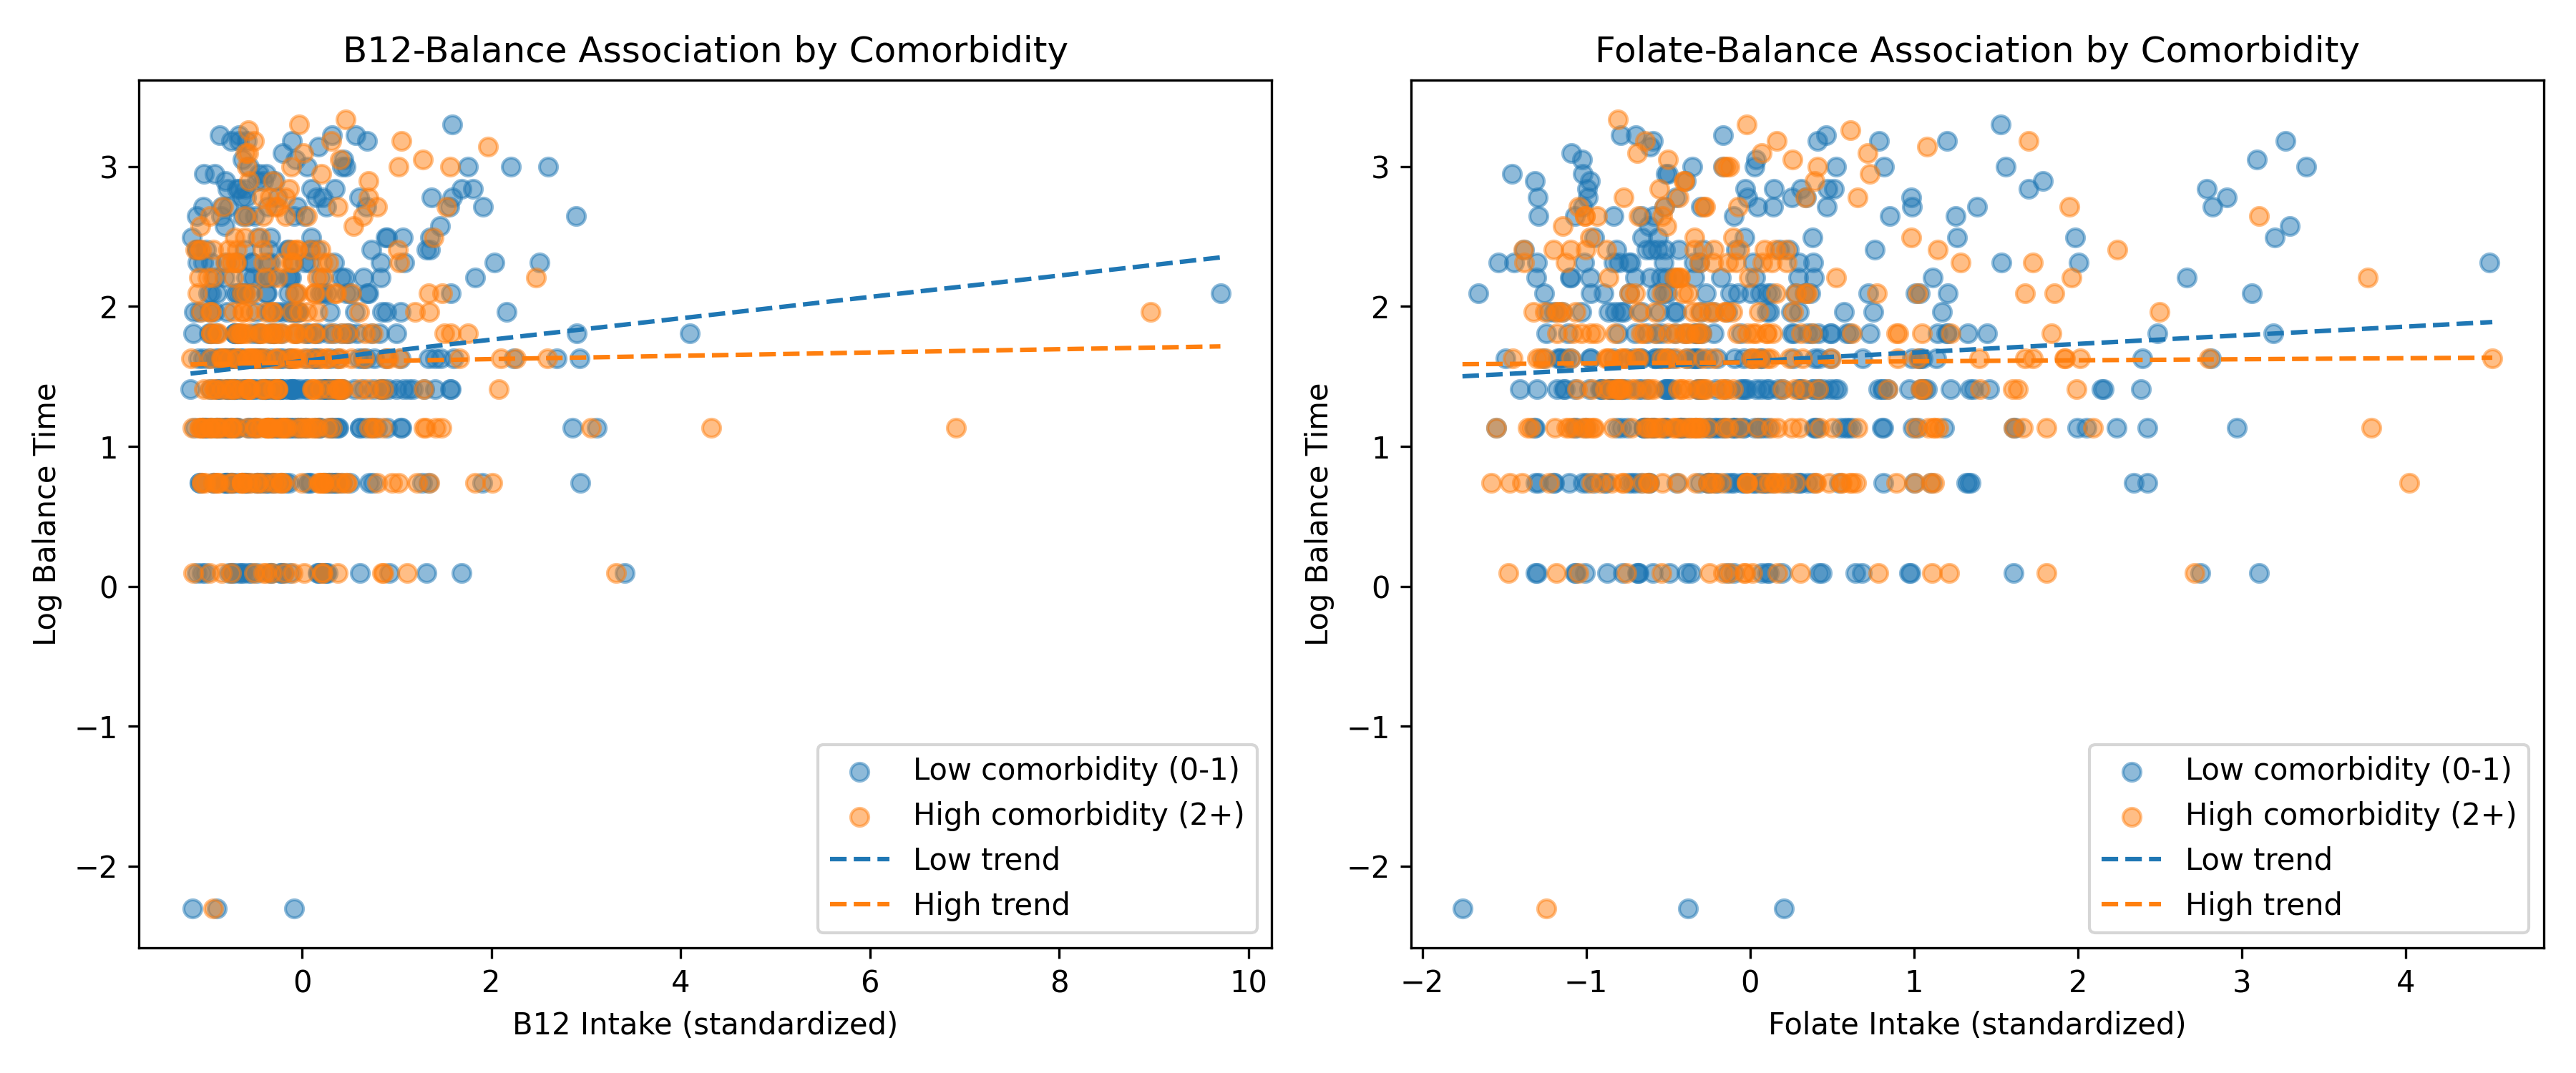
\includegraphics[width=0.85\textwidth]{../04-analysis/outputs/figures/interaction_plots.png}
\caption{Interaction plots showing the relationship between comorbidity burden and balance performance across tertiles of vitamin B12 (left panel) and folate (right panel) intake. Parallel lines indicate no significant interaction effect. Error bars represent 95\% confidence intervals.}
\label{fig:interactions}
\end{figure}

\subsection{Sensitivity Analyses}

Sensitivity analyses yielded consistent null findings. Alternative parameterizations of comorbidity burden (0/1/2+ categories vs continuous count) did not change the pattern of non-significant associations. Energy-adjusted micronutrient intake (per 1,000 kcal) produced similar null results for both B12 and folate. Excluding participants who did not meet balance readiness screening criteria (BAQ110, BAQ130) did not substantively alter the findings.

% Discussion
\section{Discussion}

\subsection{Summary of Findings}

This cross-sectional analysis of 788 older adults from NHANES cycle C (2003-2004) examined associations between comorbidity burden, dietary micronutrient intake, and objective balance performance. The primary findings were null: neither comorbidity burden nor dietary micronutrient intake (vitamin B12, folate) demonstrated significant associations with balance performance after adjusting for age, sex, and BMI. Furthermore, no significant interaction effects were observed between comorbidity burden and micronutrient intake. Age emerged as the sole significant predictor, with older age consistently associated with worse balance outcomes.

\subsection{Interpretation of Null Findings}

The absence of significant associations between comorbidity burden and balance performance contrasts with systematic review evidence linking polypharmacy to reduced physical function \cite{katsimpris2019_polypharmacy_function_review} and specific studies demonstrating polypharmacy-associated impairments in balance and mobility \cite{salkin2025_polypharmacy_balance, abubakar2021_polypharmacy_falls}. Several factors may explain this discrepancy.

First, the present study used a comorbidity count (0-3 cardiometabolic conditions) rather than a medication count as the primary exposure measure. While comorbidity and polypharmacy are correlated, medication count may capture additional dimensions of treatment burden, including central nervous system-active drugs that directly affect balance and cognition \cite{romandemettelinge2013_diabetes_falls_medications}. The specific medications used to treat chronic conditions—particularly sedatives, anticholinergics, and antihypertensives—may exert stronger effects on balance than the diseases themselves.

Second, the analytic sample represents a highly selected population of older adults who were able to complete the standardized balance examination. Individuals with severe balance impairment, advanced frailty, or cognitive limitations were likely excluded through the eligibility screening process, potentially introducing survivorship bias that attenuated associations. The final analytic sample of 788 participants represents only 45\% of age-eligible participants with balance exam data, suggesting substantial selection toward healthier, more functional individuals.

Similarly, the lack of association between dietary vitamin B12 and folate intake and balance performance diverges from findings linking B12-related metabolic pathways to physical function. Prior NHANES research documented associations between plasma homocysteine (a marker of B12/folate metabolism) and lower-extremity strength, gait speed, and physical function \cite{kositsawat2022_nhanes_hcy_function}. Observational cohort studies have demonstrated relationships between serum B12, homocysteine, and gait speed \cite{vidoni2017_b12_hcy_gait}, as well as folate status and functional disability \cite{ng2012_b12_folate_function, ji2023_nhanes_folate_disability}.

However, these studies predominantly used serum biomarkers rather than dietary intake estimates. Dietary recall data, even from validated 24-hour recalls, may not accurately reflect long-term micronutrient status or bioavailability, particularly in older adults with variable absorption due to gastric atrophy or medication use (e.g., proton pump inhibitors, metformin). The absence of supplement data in NHANES cycle C further limits the ability to capture total micronutrient exposure, as supplement use is common among older adults and may contribute substantially to B12 and folate status.

The absence of significant interaction effects between comorbidity burden and micronutrient intake suggests that, within the observed ranges of dietary intake and comorbidity, micronutrient status does not substantially modify the relationship between disease burden and balance. This finding contrasts with emerging evidence of biomarker interactions, such as the vitamin D × interleukin-6 interaction on gait speed observed in the InCHIANTI cohort \cite{kositsawat2019_vitd_il6_gait}, and highlights the importance of considering both biomarker status and inflammatory milieu in future analyses.

Age emerged as the sole significant predictor of balance performance, with each additional year of age associated with reduced balance failure time. This finding aligns with well-established age-related declines in proprioception, vestibular function, and muscle strength that collectively impair postural control \cite{talkowski2008_balance_gait_walking}. The predominance of age as a predictor may reflect that, in this relatively healthy, community-dwelling sample, chronological aging processes overshadowed the effects of comorbidity burden and dietary micronutrient intake within the observed ranges.

\subsection{Strengths and Limitations}

This study possesses several methodological strengths. First, the use of NHANES data provides a nationally representative sample of the US older adult population with rigorous standardized data collection protocols. Second, the balance examination (modified Romberg test) represents an objective, validated measure of static standing balance with established test-retest reliability. Third, the analysis incorporated NHANES survey design variables and subsample weights (WTSB2YR) to produce population-representative estimates with appropriate variance estimation. Fourth, strict data cleaning procedures were applied, including outlier removal ($|z| > 4$) and exclusion of categorical levels with limited membership ($<$5\%), reducing the influence of extreme values on regression estimates.

Several limitations must be considered when interpreting these findings. First, the \textbf{cross-sectional design} precludes assessment of temporal relationships or causality. It remains possible that poor balance precedes or co-occurs with comorbidity development and dietary changes in ways that cannot be disentangled in a single time-point analysis.

Second, \textbf{survivorship bias} represents a substantial limitation. The analytic sample was restricted to participants who completed the balance examination, which required meeting safety screening criteria. Adults with severe balance impairment, advanced frailty, or cognitive limitations were likely excluded, potentially creating a ``healthy participant'' bias that attenuated associations. This substantial attrition may have selected for healthier, more functional individuals in whom comorbidity and micronutrient effects are less pronounced.

Third, \textbf{data unavailability constrained the exposure assessment}. Vitamin D intake data was unavailable in NHANES cycle C, preventing inclusion of what may be the most relevant micronutrient for balance outcomes \cite{orces2019_nhanes_vitd_disability, kalenkoski2020_nhanes_vitd_gait, moon2019_vitd_performance}. Dietary supplement data was also unavailable, limiting micronutrient assessment to dietary intake only. Given that supplement use is widespread among older adults and contributes substantially to B12 and folate status, the failure to capture total micronutrient exposure may have introduced measurement error.

Fourth, \textbf{dietary recall limitations} apply. A single 24-hour dietary recall may not accurately reflect habitual intake, particularly for nutrients with high day-to-day variability. Additionally, the present analysis did not account for bioavailability differences or individual absorption capacity, which vary substantially in older adults due to gastric atrophy, medication use, and genetic factors.

Fifth, \textbf{the comorbidity measure was limited} to three cardiometabolic conditions (diabetes, hypertension, hypercholesterolemia). This count does not capture musculoskeletal conditions (e.g., osteoarthritis), neurological conditions (e.g., peripheral neuropathy, Parkinson's disease), or vestibular disorders that may more directly affect balance. Additionally, the comorbidity count does not account for disease severity or duration.

\subsection{Clinical and Public Health Implications}

Despite the null findings, this study carries important implications for clinical practice and public health. First, the predominance of age as a predictor of balance performance reinforces the importance of age-stratified fall risk assessment. Even in the absence of significant comorbidity burden or apparent micronutrient deficiency, advancing age itself signals elevated fall risk that warrants proactive intervention, including balance training, home safety modification, and medication review.

Second, the null findings for dietary micronutrients should not be interpreted as evidence that micronutrient status is irrelevant to balance. Rather, these findings suggest that dietary intake estimates alone may be insufficient to capture the biological exposure relevant to neuromuscular function. Clinicians should continue to assess for clinical signs of B12 and folate deficiency (e.g., macrocytic anemia, neuropathy, cognitive changes) and consider serum testing when indicated, particularly in older adults with risk factors for malabsorption.

Third, the discrepancy between comorbidity count and medication count as exposure measures highlights the importance of comprehensive medication review in older adults. While disease burden itself may not directly impair balance, the medications used to treat chronic conditions—particularly central nervous system-active drugs—may substantially increase fall risk. Deprescribing initiatives targeting potentially inappropriate medications may be more impactful for fall prevention than disease management alone.

\subsection{Future Research Directions}

This study highlights several priorities for future research:

\begin{enumerate}
    \item \textbf{Biomarker-based assessment:} Future studies should incorporate serum biomarkers of micronutrient status (B12, folate, homocysteine, 25-hydroxyvitamin D) rather than relying solely on dietary intake estimates. Biomarkers provide a more direct measure of biological exposure and account for absorption and metabolism variability.
    
    \item \textbf{Expanded NHANES cycles:} Analysis of additional NHANES cycles where vitamin D data and supplement use information are available (e.g., 2007-2014) would enable evaluation of the micronutrient most strongly linked to balance and capture total micronutrient exposure from diet and supplements.
    
    \item \textbf{Medication count vs. comorbidity count:} Direct comparison of medication-based polypharmacy measures with disease-based comorbidity counts would clarify whether medication burden, disease burden, or their combination most strongly predicts balance impairment.
    
    \item \textbf{Specific comorbidity analysis:} Rather than aggregate counts, future research should examine whether specific conditions (e.g., diabetes with peripheral neuropathy, vestibular disorders) have differential effects on balance, as these conditions may have stronger mechanistic links to postural control than cardiometabolic conditions alone.
    
    \item \textbf{Longitudinal designs:} Prospective cohort studies tracking balance change over time would enable assessment of temporal relationships and identify factors predictive of balance decline, rather than cross-sectional associations.
    
    \item \textbf{Survivorship-sensitive designs:} Studies employing inclusive recruitment strategies that capture older adults unable to complete laboratory-based balance tests—through home-based assessment or caregiver proxy report—would address the survivorship bias inherent in performance-based measures.
\end{enumerate}

% Conclusion
\section{Conclusion}

This cross-sectional study of 788 community-dwelling older adults from NHANES cycle C (2003-2004) examined associations between comorbidity burden, dietary micronutrient intake (vitamin B12, folate), and objective balance performance measured via the modified Romberg test. The primary findings were null: neither comorbidity burden nor dietary micronutrient intake demonstrated significant associations with balance performance, and no significant interaction effects were observed. Age emerged as the only significant predictor, with older age associated with worse balance outcomes.

These null findings likely reflect methodological limitations including survivorship bias, reliance on dietary intake rather than biomarker measures, and the unavailability of vitamin D and supplement data. While the present study does not support a role for dietary B12 and folate intake in balance performance within this sample, the broader literature supports continued attention to micronutrient status—particularly through biomarker assessment—and comprehensive medication review in fall prevention efforts.

The predominance of age as a predictor reinforces that balance decline is an inherent feature of aging, requiring proactive, age-stratified prevention efforts. Moving forward, research incorporating serum biomarkers, comprehensive medication assessment, longitudinal designs, and inclusive sampling will be essential to disentangle the contributions of disease burden, nutritional status, and aging itself to balance impairment in older adults.

% References
\bibliographystyle{unsrtnat}
\bibliography{../01-literature/references}

\end{document}
